\chapter{Technique Overview}\label{ch:research}
This part of the thesis constitutes the main part.
The objective create an overview of techniques in the field which may be used to solve the problem
detailed in Chapter~\ref{ch:problem}.
First the search for literature which lays the foundation for the subsequent sections, is documented.
The a taxonomy is introduced which facilitates the analization and comparison of techniques.
Lastly, the advances in the field are placed in the correct position and analyzed.

\section{Literature Search}\label{se:litSearch}
This section documents the search for literature which provides the content for the subsequent
overview.
For this, important pipelines and notable advances along with their properties are researched,
analysed and presented.
The literature is identified through searching in the Google Scholar database.
The search is executed with keywords such as but not only: Deep Learning, Text Detection,
Text Recognition, Text Spotting, Scene Text, Pipeline.
% FIXME: update keywords
A criterion for further examination is an appropriate amount of citations for the piece of literature
in question.
Additionally, literature is selected through citations for and by literature which has already been
identified as important.
All research after 2018 which pertains to extracting scene text is regarded as relevant.
Standard \ac{OCR} solutions may not hold validity in practice, as the image and text conditions can
vary in the defined problem~\citep{chen_text_2021}.
The delimination from Section~\ref{se:problem} of course holds for this chapter and only literature
which concerns advances for the \ac{DL} model will be regarded as important for the scope of this
thesis.
This extends to the whole pipeline from preprocessing an image to the final result of the model.

% FIXME: hierarchical graphic with found papers
% FIXME: describe proceeding

\section{Taxonomy of Pipeline Steps}
In order to create the overview the necessary steps in the process of \ac{STS} need to be highlighted,
from preprocessing to classifying the identified text~\citep{long_scene_2021, sourvanos_challenges_2018}.
The ways in which the respective issues for the steps are solved are identified from literature,
listed and explained alongside.

\begin{itemize}
    \item Bestandteile nicht zwangsweise sequentiell
    \item Tiefe: Pipeline Steps
        $\rightarrow$ possible solutions
        $\rightarrow$ research points (only mention)
        e.g.: Sequence Modeling $\rightarrow$ CNN, RNN, Transformer $\rightarrow$ \ldots
    \item Lexicon Free Models!
    \item Trend: detection moves towards segmentation, recognition away
\end{itemize}

\begin{comment}
    - What is segmentation
    - Detection: from pixel to character -> better for arbitrary shapes
        - Segmentation
        - Text detection of of segmentation
    - Recognition: are not used often (poor word-level results)
        - Segmentation
        - recognition
    - End to end?
\end{comment}

\tikzset{
    font=\scriptsize,
    edge from parent fork down,
    level distance=1.75cm,
    every node/.style={
            top color=white,
            bottom color=blue!25,
            rectangle,rounded corners,
            minimum height=6mm,
            draw=blue!75,
            very thick,
            drop shadow,
            align=center,
            text depth = 0pt,
    },
    edge from parent/.style={draw=blue!50,thick}
}

\begin{figure}[ht]
    \centering
    \begin{tikzpicture}
        \Tree [.STS
            [.{STD}
                [.{Feature \\ Extraction} ]
                [.{BB Regression} ]
            ]
            [.{STR}
                [.{Preprocessing} ]
                [.{Feature \\ Extraction} ]
                [.{Sequence \\ Modelling} ]
                [.{Prediction} ]
            ]
        ]
    \end{tikzpicture}
\caption{Pipeline steps with increasing granularity\label{fig:pipelineSteps}}
\end{figure}

\begin{figure}[h]
    \centering
    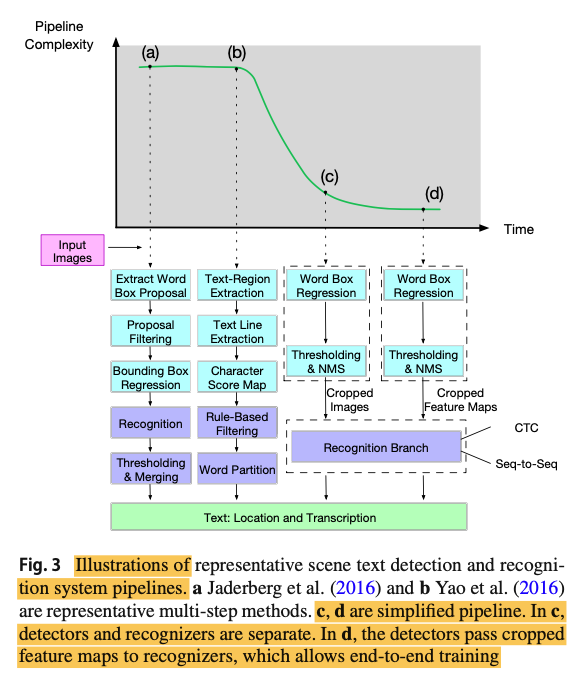
\includegraphics[width=0.80\textwidth]{img/Long-Scene-2021-Pipeline-Changes.png}
    \caption{Pipeline changes~\citep{long_scene_2021}\label{fig:piplineChanges}}
\end{figure}

\begin{figure}[h]
    \centering
    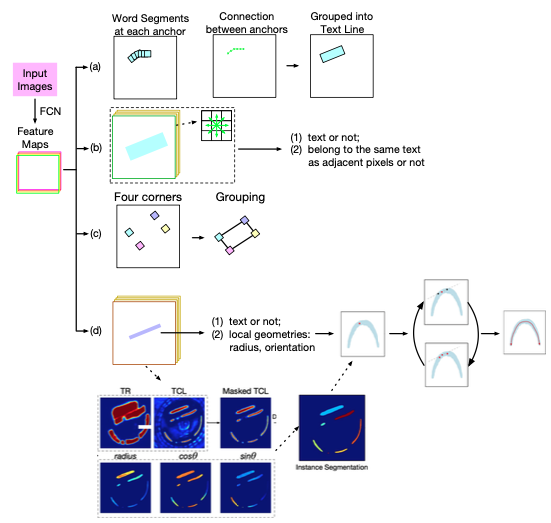
\includegraphics[width=0.80\textwidth]{img/Long-Scene-2021-STD-Pipelines.png}
    \caption{STD pipelines~\citep{long_scene_2021}\label{fig:STD-pipelines}}
\end{figure}

\begin{figure}[h]
    \centering
    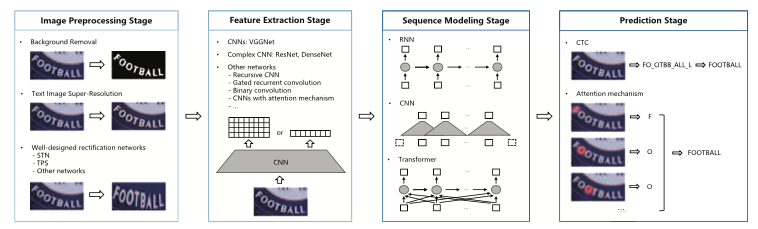
\includegraphics[width=0.95\textwidth]{img/Chen-Text-2021-STR-Pipeline.png}
    \caption{STR pipeline~\citep{chen_text_2021}\label{fig:STR-pipeline}}
\end{figure}
Same pipeline for~\cite{baek_what_2019}


\begin{itemize}
    \item For Detection: describe how BB is assigned to ground truth while training \& testing
\end{itemize}

An accurate Segmentation-Based \ldots~\citep{liu_accurate_2020}
\begin{itemize}
    \item For detection there's two categories: detection-based, segmentation based
        $\rightarrow$ latter is more getting more popular
        \begin{itemize}
            \item detection-based: adapt general object detection framework
                $\rightarrow$ directly regress quadrangles
                $\rightarrow$ problem with arbitrary shapes and small texts
            \item segmentation-based: use pixel-wise segmentation to segment text areas
                $\rightarrow$ use segment text areas to extract text instances by post-processing
        \end{itemize}
    \item look into paper for overview of text detection
    \item Text Detection is type of object detection
\end{itemize}

Scene Text Detection and Recognition~\cite{long_scene_2021}
Deep learning $\rightarrow$ frees researchers from hand-crafting features, simplifies pipeline,
    improves performance

Difference: two-part pipeline vs end-to-end
\begin{itemize}
    \item two-part / Detection \& Recognition: detector passes cropped image to recognizer
    \item end-to-end: detector passes cropped feature maps to recognizer $\rightarrow$ end-to-end
            training
\end{itemize}

\textbf{Text detection and localization}
can be generalized under object detection --- generally: one-staged or two staged methods
scene text detection algorithms often inspired bz object detectors --- difference:
        text is homogeneous as a whole and characterized bz its locality
stages of development
\begin{itemize}
    \item early DL approaches: long and slow pipelines, design methodology is bottom up
    \item methods inspired by object detection:
        \begin{itemize}
            \item modifying region proposal and bounding box regression modules to localize text
                directliy
            \item consist of stacked convolutional layers that encode image into feature maps
            \item spatial location at the feature maps corresponds to region of input image
            \item feature maps are fed into classifier for prediction of existance and localization
        \end{itemize}
        see p.5 / p.165 for specific papers
    \item Methods based on Sub-text components
        \begin{itemize}
            \item any part of a text insance is still text
                $\rightarrow$ only predict sub-text components and then assemble into a text instance
            \item use NN to predict local attributes or segments $\rightarrow$ postprocessing for
                re-construction
            \item in comparison to early DL-approaches: rely more on NN and shorter pipelines
            \item different approaches
                \begin{itemize}
                    \item pixel-level: learn dense prediction map --- does pixel belong to
                        any text instances
                    \item component-level: predict local region of text instance (overlapping one or
                        more characters)
                    \item character-level: learn segmentation map for character centers and links
                        between them, centers and links predicted in form of gaussian heat map,
                        problem: requires iterative weak supervision, but real-world datasets rarely
                        equipped with character-level labels
                \end{itemize}
                sub-text components: \\
                better flexibility and generalization over shapes and aspect ratios\\
                drawback: module or post-processing step used to group segments into text instances
                may be vulnerable to noise and the efficiency
        \end{itemize}
\end{itemize}

\textbf{Recognition --- Text transcribing and converting into linguistic symbols}
use CNNs to encode images into feature space
different approaches in text content decoding module:
challenge: represent oriented characters and curved text that are distributed over a 2-dimensional space
    (rather than 1-dim/horizontal) in order to fit decoding modules (whose decodes require
    1-dimensional inputs)
\begin{itemize}
    \item Connectionist Temporal Classification (CTC)
        \begin{itemize}
            \item input images are viewed as sequence of vertical pixel frames
            \item network outputs per-frame prediciton $\rightarrow$ probability distribution of
                label types for each frame
            \item CTC-rule is applied to edit per-frame prediction to a text string
            \item training end-to-end: sum of negative log propability of all possible per-frame
                predictions that generate target sequence by CTC-rules
            \item less dependant on language models and has better character to pixel alignment
        \end{itemize}
    \item Encoder-Decoder Framework
        \begin{itemize}
            \item encoder RNN reads input sequence and passes final latent state to decoder RNN
                which generates output in auto-regressive way
            \item often combined with attention mechanism
            \item decoder is an implicit language model: can incorporate more linguistic priors
        \end{itemize}
    \item adaptions for irregular text recognition
        \begin{itemize}
            \item Spatial Transformer Networks (predict text bounding polyglons with fc-layers for
                thin-plate-spline transformations to rectify irregular input into more canonical form)
                $\rightarrow$ Sequence Recognition Network
            \item \ldots
        \end{itemize}
    \item other methods
        \begin{itemize}
            \item perform word recognition by classifying image into pre-defined set of vocabulary
            \item improve occlusion cases: transformer-based semantic reasoning module
        \end{itemize}
\end{itemize}
evaluation of recognition methods falls behind the time robustness of recognition when cropped
with slightly differend bounding box is seldom verified

\textbf{End-to-end system}
also known as text spotting systems, profiting from idea of designing differentiable computation graphs
\begin{itemize}
    \item Two-step pipeline:
        \begin{itemize}
            \item recent work goes away from character level and towards word or line level
            \item first generate proposal using text detection model, thenrecognize using
                text recognition model
            \item detected words are cropped from the image $\rightarrow$ detection and recognition
                are two separate steps
        \end{itemize}
    \item Two-stage pipeline
        \begin{itemize}
            \item more recent
            \item cropp feature maps instead of images and feed to recognition modules
        \end{itemize}
    \item One-Stage Pipeline:
        \begin{itemize}
            \item predict character, text bounding boxes and character type segmentation
                maps in parallel
            \item text bb are used to group character boxes to form final word transcription results
        \end{itemize}
\end{itemize}

Challenges in input preprocessing for mobile OCR applications~\cite{sourvanos_challenges_2018}
from 2018 $\rightarrow$ outdated
\begin{itemize}
    \item Acquistion: obtaining image --- digitization, binarization, compression
    \item Preprocessing: enhancing image quality --- noise removal, skew removal, thinning,
        morphological operations
    \item Segmentation: separating structural elements --- implicit and explicit segmentation
    \item Feature extraction: generating salient features --- geometrical, statistical
    \item Classification: categorizing individual characters to their respective classes --- clustering,
        neural networks, bayesian models, etc.
    \item Post-processing: improving and filtering --- contextual approaches, multiple classifiers, dictionary based approaches
\end{itemize}

Text Recognition in the Wild: A Survey~\citep{chen_text_2021}
various stages of \ac{OCR}:
\begin{itemize}
    \item text localization: localize text components, group into candidate text regions with
        as little background as possible, DNN
    \item text verification: verify text candidate regions as text or non-text,
        filter false-positives, CNN
    \item text detection: determine whether text is present using localization and verification
        procedures, basis for end-to-end, can be regression or segmentation based\\
        $\rightarrow$ regression based or segmentation based
    \item text segmentation: most challenging, includes text line (splitting a region of multiple
        text lines into subregion of single text lines) and character segmentation (separating
        text instance into single characters, typically used in earlier approaches)
    \item text recognition: translates cropped text instance image into target string sequence,
        basis for end-to-end, DL encoder-decoder frameworks
    \item end-to-end-system: given scene text image $\rightarrow$ convert all text regions into
        target string sequences, includes detectoin, recognition and postprocessing, can be
        seen as indipendent subproblems but also joint by sharing information
\end{itemize}

text enhancement: recover degraded text, improve text resolution, remove distortions,
remove background $\rightarrow$ reduce difficulty of recognition

Cropped Scene Text Image Recognition
\begin{itemize}
    \item Main categories: Segmentation-based --- Segmentation-free \\
        Segmentation-based
        \begin{itemize}
            \item Approach: locate position of character, apply chlassifier to recognize each character,
                group characters into text lines
            \item substeps: image preprocessing, character segmentation, character recognition
            \item lexicon methods: query time linearly depends on size of lexicon
                $\rightarrow$ impractical --- solve: higher-order statistical language models
            \item lexicon-free methods: leverage more data and more complex NN
            \item Shortcommings: require accurate character detection (hard), fail to model contextual
                information beyond individual characters $\rightarrow$ poor word-level results
                during training
        \end{itemize}
        Segmentation-free
        \begin{itemize}
            \item approach: recognize text line as a whole and focus on mapping entire text instance
                image into target string sequence
            \item stages:
                \begin{itemize}
                    \item Preprocessing: improve image quality\\
                        background removal: separate text from complex backgrounds\\
                        super-resolution: TextSR can output plausible high-resolution image\\
                        rectification: remove distortion (perspective and curving shape) STN, TPS
                    \item Feature extraction: various CNN backbone networks (VGG, ResNet, Binary Conv)\\
                        maps image to representation that reflects attributes relevant for OCR, while
                        suppressing irrelevant features\\
                        Deeper and more advanced extractor better, but higher performance cost
                    \item Sequence Modeling: RNN, CNN, Transformer \\
                        bridge between visual features and predictions, capture contextual informtion
                        within sequence of characters, helpful as it is more stable than treating each
                        symbol independently\\
                        often BiLSTM because of ability to capture long-range dependencies
                        problem: computationally expensive, time consumine, gradient vanishing/exploding
                        deep one dimensional CNN instead of BiLSTM\\
                        transformer structure
                    \item Prediction stage: estimate target string from features\\
                        CTC
                        attention-based
                        CRNN also an option but more 2017 $-$ 2018
                        Look into: aggregation cross-entropy functiona
                            $\rightarrow$ replace CTC and attention mechanism
                \end{itemize}
        \end{itemize}
        Other approaches
        \begin{itemize}
            \item
        \end{itemize}
\end{itemize}

CTC
\begin{itemize}
    \item for training RNNs to label unsegmented sequences directly
    \item transcription layer converts input features by CNNs or RNNs into target string sequence
        by calculating conditional probability
    \item efficiently sum over all possible input-output sequence alignments and allow classifier
        to be trained without any prior alignment between input and target sequences
    \item is adapted to forward-backward algorithm for efficient computation
    \item problem:
        \begin{itemize}
            \item produces highly peaky and overconfident distributions $\rightarrow$ overfitting
                $\rightarrow$ regularization to enhance generalization and exploration capabilities
            \item large computational cost for long text sequences
            \item can hardly be applied to two-dimensional prediction problems (text distributed
                in a spatial structure)
        \end{itemize}
\end{itemize}
Attention-Based
\begin{itemize}
    \item for STR often combined with RNN structure
    \item learns alignment between input instance image and output text sequences by referring
        to the history of the target characters and the encoded feature vectors
    \item outperform CTC in decoding because of ability to focus in informative areas
    \item can be extended to complex 2D prediction problems
    \item higher accuracy on isolated word recognition but perform worse on sentence tasks
        when compared to CTC
    \item problems
        \begin{itemize}
            \item attention modul for label alignment $\rightarrow$ storage and compuation
            \item attention drift phenomenon: for long text sequences, attention mechanism is difficult
                to train from scratch owing to misalignment between input instance image and output
                text sequences
            \item current research mainly focuses on few character categories (chinese might be bad)
        \end{itemize}
\end{itemize}

End-to-end Systems
\begin{itemize}
    \item directly convert all text regions into string sequences
    \item includes text detection, text recognition and postprocessing
    \item reasons for end-to-end
        \begin{itemize}
            \item real-time and efficient
            \item errors can accumulate in cascade way for detection and recognition, end-to-end
                can prevend accumulation during training
            \item end-to-end system can jointly be optimized
            \item easier to maintain and adapt to new domains
            \item competitive performance with faster interference and smaller storage requirements
        \end{itemize}
\end{itemize}


What is wrong with scene text recognition model comparison~\cite{baek_what_2019}
Four stages derived from existing STR-Models --- \textbf{only recognition}
\begin{itemize}
    \item Transformation: normalize input image $\rightarrow$ Spatial Transormer Network
        \begin{itemize}
            \item transform input image $X$ into $\tilde{X}$
            \item if curved and tilted texts / other diverse shapes are forwarded unaltered,
                feature extraction needs to learn an invariant representation
            \item thin-plate spline transformatino (variant of spatial transformation network)
                $\rightarrow$ smooth spline interpolation between set of fiducial points
        \end{itemize}
    \item Feature extraction: map input image to representation that focuses on relevant attributes,
        while suppressing irrelevant features
        \begin{itemize}
            \item use \ac{CNN} to abstract image $\tilde{X}$ to output visual feature map
                $V=\{v_i\}, i=i,\ldots,I$\\
                I is number of columns in feature map, each column has a corresponding distinguishable
                receptive field along the horizontal line of $\tilde{X}$
            \item important architectures: VGG, RCNN, ResNet
        \end{itemize}
    \item Sequence Modeling: capture contextual information within sequence of characters
        \begin{itemize}
            \item reshape extracted featured to be a sequence of features $V$ (each column)
            \item use Bidirectional LSTM $\rightarrow$ sequence $H=Seq.(V)$
            \item this stage is optional
        \end{itemize}
    \item Prediction: estimate output character sequence
        \begin{itemize}
            \item use $H$ to predict a sequence of characters $Y=y_1,y_2,\ldots,y_n$
            \item options: Connectionist temporal classification or attention-based sequence prediction
        \end{itemize}
\end{itemize}
Tradeoff:
\begin{itemize}
    \item accuracy-speed
    \item accuracy-memory
\end{itemize}

Some part for which datasets have which characteristics? see~\cite{long_scene_2021}

\section{State of the Art Methods}

text enhancement:~\cite{chen_text_2021}
model pruning:~\cite{niu_26ms_2019}
integer inference:~\cite{ignatov_ai_2019}
